\documentclass{paper}

\usepackage{amsmath,lstautogobble,amssymb,amsfonts, listings, fancyhdr, stmaryrd, array, tikz}
\usepackage[many]{tcolorbox}
\usepackage[T1]{fontenc}
\usepackage[utf8]{inputenc}
\usepackage[a4paper, total={170mm,257mm}, left=20mm, top=20mm]{geometry}
\usepackage{adjustbox}
\definecolor{color0}{HTML}{000000}
\definecolor{color1}{HTML}{000000}
\definecolor{bgColor}{HTML}{ffffff}
\usetikzlibrary {arrows.meta,bending} 

\newtheorem{prop}{Proposition}
\newtheorem{definition}{Definition}
\newtheorem{preuve}{Preuve}

\definecolor{codegreen}{rgb}{0,0.6,0}
\definecolor{codegray}{rgb}{0.5,0.5,0.5}
\definecolor{codepurple}{rgb}{0.58,0,0.82}
\definecolor{backcolour}{rgb}{0.95,0.95,0.92}
\lstdefinestyle{mystyle}{
    language=caml,
    backgroundcolor=\color{backcolour},   
    commentstyle=\color{codegreen},
    keywordstyle=\color{magenta},
    numberstyle=\tiny\color{codegray},
    stringstyle=\color{codepurple},
    basicstyle=\ttfamily\footnotesize,
    breakatwhitespace=false,         
    breaklines=true,                 
    captionpos=b,                    
    keepspaces=true,                 
    numbers=left,                    
    numbersep=5pt,                  
    showspaces=false,                
    showstringspaces=false,
    showtabs=false,                  
    tabsize=2,
    autogobble=true
}

\lstset{style=mystyle}

\newcolumntype{C}{>$c<$}
\tcolorboxenvironment{prop}{enhanced, borderline={0.8pt}{0pt}{blue}, borderline={0.4pt}{2pt}{cyan}, boxrule=0.4pt, colback=white, coltitle=black, sharp corners}
\tcolorboxenvironment{definition}{ enhanced, borderline={0.8pt}{0pt}{red}, borderline={0.4pt}{2pt}{orange}, boxrule=0.4pt, colback=white, coltitle=black, sharp corners}
\tcolorboxenvironment{preuve}{ enhanced, borderline={0.8pt}{0pt}{green}, borderline={0.4pt}{2pt}{lime}, boxrule=0.4pt, colback=white, coltitle=black, sharp corners}

\pagestyle{fancy}
\fancyhead[C]{TIPE 25/26 - Dorian GIL}

\begin{document}
\setlength{\headheight}{13.07225pt}
\addtolength{\topmargin}{-1.07225pt}

\section*{Model Checking et LTL: Application de la méthode des tableaux et de l'algorithme de Gerth}

\tableofcontents


\section{Introduction}
Dans un monde dont la dépendance à divers technologies est très importante, il est important de s'assurer du bon fonctionnement de ces technologies.
C'est ainsi que la vérification de modèle rentre en jeu pour répondre à ces problèmatiques. La vérification de problème requiert des algorithmes permettant justement de faire ces vérifications...
C'est donc dans le cadre de la logique temporelle linéaire appliqué à la vérification de modèle, que nous allons examiner les deux méthodes décrites plus tard.


\section{Préliminaires}

\subsection{Model Checking et LTL}

    \begin{definition}[Formule de la LTL]
        On définit $F$ l'ensemble des formules de la LTL inductivement par:
        \begin{itemize}
            \item $p\in AP \implies p\in F$
            \item si $\psi$ et $\phi$ sont des formules de LTL alors $\lnot\psi, \phi\lor\psi, X\psi, \phi U\psi$ sont des formules de LTL
        \end{itemize}
        $AP$ un ensemble fini de variables propositionnelles.
    \end{definition}
    \begin{definition}[Opérateurs X et U]
        On les définit par:
            \begin{itemize}
                \item $X\phi$ : $\phi$ doit être satisfaite dans l'état suivant (neXt)
                \item $\psi U\phi$ : $\psi$ doit être satisfaite dans tous les états jusqu'à un état où $\phi$ est satisfait (Until)
            \end{itemize}
        \end{definition}


    \begin{definition}[Monde]
        On définit un tel objet comme $\omega := w_0,w_1,\dots$ une suite infinie d'état.
        On écrira $\omega^i:=w_i,w_{i+1},\dots$ un suffixe de $\omega$.
    \end{definition}
    Soit $v : \omega\times F \rightarrow \{T,F\}$ une fonction de valuation.
    \begin{definition}[Satisfaction d'un monde]
        En LTL, on définit $\omega \models f$ via:
        \begin{itemize}
            \item $\omega \models a \Leftrightarrow v(w_0,a) = T$ si $a$ atomique 
            \item $\omega \models \lnot f$ si $\lnot(\omega \models f)$ 
            \item $\omega \models f\lor g$ si $\omega \models f$ ou $\omega \models g$
            \item $\omega \models \textbf{X}f$ si $\omega^1 \models f$
            \item $\omega \models f\textbf{U}g$ si $\omega \models g$ ou $\omega \models f\land\textbf{X}(f\textbf{U}g)$
        \end{itemize}
    \end{definition}

    On peut trouver plusieurs applications à la LTL:
    \begin{itemize}
        \item Preuve de programme concurrentiel
        \item Raisonnement sur des circuits intégrés
        \item Raisonnement sur les protocoles de communications
    \end{itemize}
    Toutes ces applications s'inscrivent dans le cadre de la vérification de modèles qui est une méthode permettant de montrer
    la correction de systèmes informatiques complexes.

    \begin{definition}[Verification de modèle (Model Checking)]
        Technique de vérification qui explore tout les états possible d'un système de manière force brute.
    \end{definition}

    \begin{itemize}
        \item Ce n'est pas avec la LTL que nous allons faire des gros exemples de model checking (Un model checker de base peut s'occuper de $10^9$ états environ, allant jusqu'à $10^{476}$ pour les meilleurs!).
        \item Ainsi un model checker typique pourrait utiliser entre autres la LTL pour s'occuper en particulier des deadlocks. C'est ainsi qu'on pourrait utiliser la méthode des tableaux pour prouver une formule qui montre
            que des algorithmes vont bien s'executer de manière à ne pas avoir d'inter-dépendance.
        \item Ainsi nous allons examiner un exemple dans lequel nous allons appliquer la méthode des tableaux pour prouver le bon fonctionnement du système choisit!
    \end{itemize}    

\subsection{Méthode des tableaux}

    \begin{definition}[Méthode des tableaux]
        Algorithme pour prouver qu'une assertion $\phi$ ayant pour hypothèse $(H_n)$ soit satisfiable
    \end{definition}
    On supposera que aucune hypothèse n'est faite, on peut facilement adapter l'étude que l'on va faire lors d'ajout d'hypothèse.
    \begin{itemize}
        \item On place $\phi$ et ses hypothèses dans la racine.
        \item On applique des règles $(R_x)$ à chaque formule en bout d'arbre qui sont developpables
        \item Si on trouve des contradictions (des \textit{cycles}) dans toutes les branches de l'arbre (branches fermées), l'arbre est fermé donc la formule est insatisfiable.
    \end{itemize}
    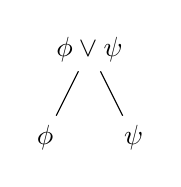
\begin{tikzpicture}[scale=0.75]
    \node {$\phi\lor\psi$}
        child {node {$\phi$}}
        child {node {$\psi$}};
    \end{tikzpicture}
    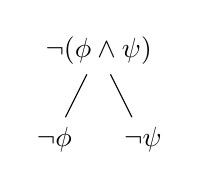
\begin{tikzpicture}[scale=0.75]
    \node {$\lnot(\phi\land\psi)$}
        child {node {$\lnot\phi$}}
        child {node {$\lnot\psi$}};
    \end{tikzpicture}
    \begin{tikzpicture}[scale=0.75]
    \node {$\lnot\lnot\phi$}
        child {node {$\phi$}};
    \end{tikzpicture}
    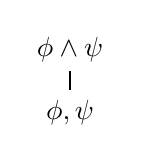
\begin{tikzpicture}[level distance=8mm]
    \node {$\phi\land\psi$}
        child {node {$\phi, \psi$}};
    \end{tikzpicture}  
    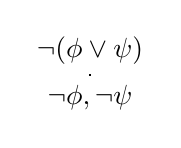
\begin{tikzpicture}[level distance=8mm,scale=0.75]
    \node {$\lnot(\phi\lor\psi)$}
        child {node {$\lnot\phi, \lnot\psi$}};
   \end{tikzpicture}


    Les règles définis précedemment sont dites Smullyan-Style

    \begin{definition}[Branche fermée]
        Une branche est fermée si elle contient $\phi$ et $\lnot\phi$
    \end{definition}
    Une formule est insatisfisable ssi son arbre associé est dit fermé ssi toutes les branches le sont.

    On peut utiliser la méthode des tableaux pour montrer qu'une formule est une tautologie:
    \begin{enumerate}
        \item On place $\lnot\phi$ et ses hypothèses dans la racine.
        \item On applique des règles $(R_x)$ à chaque formule en bout d'arbre qui sont developpables
        \item Si on trouve $a$ et $\lnot a$ dans les branches de l'arbre (des \textit{cycles}), alors $\phi$ est une tautologie
    \end{enumerate}
    On pourra donc aussi adapter nos recherches pour la recherche de tautologie.
    \begin{itemize}
        \item On ajoute les quantificateurs $\exists$ et $\forall$
        \item Un ensemble de fonctions de symboles $\mathcal{F}$ qui a des symboles associe un symbole
        \item Un ensemble de relation $\mathcal{R}$ qui a des symboles associe un booléen.
    \end{itemize}
    On note l'arité le nombre d'argument d'une fonction et $X$ les variables.
    \begin{definition}
        On définit les termes $\mathcal{T}(\mathcal{F}, X)$ par induction:
        \begin{itemize}
            \item Tout $x\in X$ est un terme.
            \item Les constantes sont des termes (symbole d'arité 0).
            \item $f(t_1,\dots, t_n)$ est un terme si $f$ est un symbole d'arité $n$ et $t_1,\dots,t_n$ sont des termes.
        \end{itemize}
    \end{definition}
    On ajoute quatres règles pour le 1er ordre (?):

    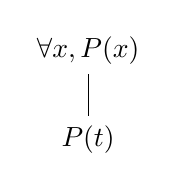
\begin{tikzpicture}[scale=0.75]
    \node {$\forall x, P(x)$}
        child {node {$P(t)$}};
    \end{tikzpicture}
    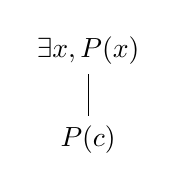
\begin{tikzpicture}[scale=0.75]
    \node {$\exists x, P(x)$}
        child {node {$P(c)$}};
    \end{tikzpicture}
    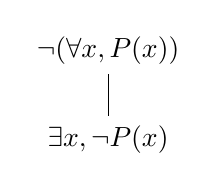
\begin{tikzpicture}[scale=0.75]
    \node {$\lnot(\forall x, P(x))$}
        child {node {$\exists x, \lnot P(x)$}};
    \end{tikzpicture}
    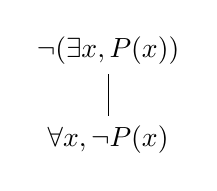
\begin{tikzpicture}[scale=0.75]
    \node {$\lnot(\exists x, P(x))$}
        child {node {$\forall x, \lnot P(x)$}};
    \end{tikzpicture}
    
    où $t$ et $c$ est une variable fixe quelquonque.
    
    \textbf{Attention:} Pour la règle $\forall$, on peut choisir $t$, pour la règle $\exists$, on prend une variable fraiche $c$!


    On définit deux nouvelles règles pour la méthode des tableaux en LTL:

    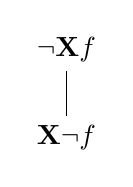
\begin{tikzpicture}[scale=0.75]
    \node {$\lnot\textbf{X}f$}
        child {node {$\textbf{X}\lnot f$}};
    \end{tikzpicture}
    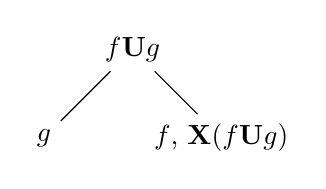
\begin{tikzpicture}[scale=0.75, level 1/.style={sibling distance=3cm}]
    \node {$f\textbf{U}g$}
        child {node {$g$}}
        child{node {$f$, $\textbf{X}(f\textbf{U}g)$}};
    \end{tikzpicture}
    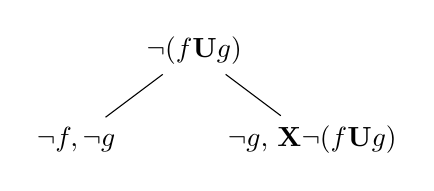
\begin{tikzpicture}[scale=0.75, level 1/.style={sibling distance=4cm}]
    \node {$\lnot(f\textbf{U}g)$}
        child {node {$\lnot f, \lnot g$}}
        child{node {$\lnot g$, $\textbf{X}\lnot(f\textbf{U}g)$}};
    \end{tikzpicture}

    \begin{definition}[Formule élementaire]
        $f$ est élementaire ssi il respecte un de ses 2 points:
        \begin{itemize}
            \item C'est une formule atomique (ou la négation d'une formule atomique)
            \item Il a comme connecteur logique "principale" $\textbf{X}$ (des X-formules)
        \end{itemize}
    \end{definition}
    Si un noeud contient uniquement des formules elementaires, alors on créé un fils
    du noeud contenant toutes les \textbf{X}-formules sans leur connecteur logique principal $\textbf{X}$


\subsection{Automate de Buchi}

    \begin{definition}[BA]
        Un automate de Büchi est un 5-uplets $(S, I, T, F, \Sigma)$ tel que
        \begin{itemize}
            \item $S$ est un ensemble fini d'état
            \item $I\subseteq S$ un ensemble d'état initiaux
            \item $F\subseteq S$ un ensemble d'état finaux
            \item $\Sigma$ Un ensemble fini de symboles appelé alphabet
            \item $T: \{S\times \Sigma\}\mapsto \mathcal{P}(S)$ Une fonction de transition.
        \end{itemize}
        Cet automate particulier accepte des séquences infinis (donc des mots infinis) ssi le mot passe par un état acceptant une infinité de fois.
    \end{definition}
    C'est un outil utilisé dans le cadre de la vérification de modèle en LTL.
    

    On va utiliser l'algorithme de Gerth pour transformer notre formule LTL en Automate de Büchi Généralisé (GBA)
    \begin{definition}[GBA]
        Un GBA est un automate de Büchi avec la seule particularité que $F$ est un ensemble d'ensemble d'état acceptant appelé \textbf{condition d'acceptation}.
        
        Un GBA accepte un mot ssi il est passé une infinité de fois par un état dans chaque ensemble d'état acceptant.
    \end{definition}
    Nous nous ramenerons à un Automate de Büchi via un autre algorithme pour simplifier.


    Un ensemble multiple d'état acceptant peut être traduit en un ensemble en construisant un automate par une "counting construction". 
    C'est à dire si $A = (S,I, \{F_1,\dots,F_n\}, \Sigma, T)$, alors il est equivalent à $A' = (S',I', F, \Sigma, T')$ telle que
    \begin{itemize}
        \item $Q' = Q\times\{1,...,n\}$
        \item $I' = I\times\{1\}$
        \item $F'=F_1\times \{1\}$
        \item $\Delta' = \{ ( (q,i), a, (q',j) ) | (q,a,q') \in \Delta$ et si $q \in F_i$, $j= i+1 \mod n$ sinon $j=i \}$
    \end{itemize}
    qui est bien un automate de Büchi.

\begin{definition}[Intersection de BA]
    On définit l'automate reconnaissant l'intersection de deux langages comme $A'= (S', I', F', \Sigma, T')$ telle que
    \begin{itemize}
        \item $S'=S_1\times S_2\times \{1,2\}$
        \item $T'=T_1'\cup T_2'$
        \begin{itemize}
            \item $T_1=\{((q_1,q_2,1),a,(q_1',q_2',i)), (q_1,a,q_1')\in T_1, (q_2,a,q_2')\in T_2, q_1\in F_1 \Leftrightarrow i= 2, i\in[|1,2|]\}$
            \item $T_2=\{((q_1,q_2,2),a,(q_1',q_2',i)), (q_1,a,q_1')\in T_1, (q_2,a,q_2')\in T_2,  q_2\in F_2 \Leftrightarrow i= 1, i\in[|1,2|]\}$
        \end{itemize}
        \item $I'= I_1\times I_2 \times \{1\}$
        \item $F'= \{(q_1,q_2,2), q_2\in F_2 \}$
    \end{itemize}
\end{definition}

\begin{definition}[Test BA Vide]
    Un BA est non vide ssi il existe un état final qui est atteignable depuis un état initial et appartient à un cycle.
    
    Pour cela on considère notre automate comme un graphe orienté, qu'on décompose en CFC, puis on fait un DFS depuis les etats initiaux et on trouve une CFC non trivial tq il contient un etat final et est atteignable par un état initial.
\end{definition}

\begin{definition}[GBA2BA]
    Un ensemble multiple d'état acceptant peut être traduit en un ensemble en construisant un automate par une "counting construction". 
    C'est à dire si $A = (S,I, \{F_1,\dots,F_n\}, \Sigma, T)$, alors il est equivalent à $A' = (S',I', F, \Sigma, T')$ telle que
    \begin{itemize}
        \item $Q' = Q\times\{1,...,n\}$
        \item $I' = I\times\{1\}$
        \item $F'=F_1\times \{1\}$
        \item $\Delta' = \{ ( (q,i), a, (q',j) ) | (q,a,q') \in \Delta$ et si $q \in F_i$, $j= i+1 \mod n$ sinon $j=i \}$
    \end{itemize}
    qui est bien un automate de Büchi (non généralisé).
\end{definition}

\subsection{Résumé}
    Pour résumé, nous devons faire:
    \begin{enumerate}
        \item Implémentation de la méthode des tableaux en LTL
        \item Implémentation des automates de Büchi
        \begin{itemize}
            \item Implémentation des bases
            \item Implémentation de l'algorithme de Gerth
            \item Implémentation de la traduction entre GBA et BA
        \end{itemize}
        \item Vérification de modèle en utilisant les 2
    \end{enumerate}

    Ensuite, nous mettrons cela en application sur la vérification du bon fonctionnement d'un feu rouge. Nous donnerons une formule logique définissant son clignotement et nous vérifirons via
    la méthode des tableaux que la formule est correcte selon ce qu'on attend d'elle. Et nous ferons de même avec l'automate de Buchi.

\begin{adjustbox}{center}
\begin{tikzpicture}
\tikzset{x=1ex,y=1ex} 
\clip (0,0) rectangle (85.50, 47.44);
\fill[bgColor] (0,0) rectangle (85.50, 47.44);
\node[color=color0, anchor=north west, scale=0.8, rotate=0.00, text width=2.12cm] at (33.39, 41.71) {Vérification};
\draw[line width=1.24pt, color=color0, ] (29.94, 29.27) -- (33.92, 37.52);
\draw[line width=1.24pt, color=color0, ] (50.67, 29.27) -- (46.52, 37.57);
\node[color=color0, anchor=north west, scale=0.8, rotate=0.00, text width=2.69cm] at (23.87, 29.03) {Automate $A_m$};
\node[color=color0, anchor=north west, scale=0.8, rotate=0.00, text width=3.66cm] at (44.60, 28.89) {Automate $A_{\lnot(\varphi)}$};
\draw[line width=1.24pt, color=color0, ] (38.23, 20.98) -- (29.94, 25.13);
\draw[line width=1.24pt, color=color0, ] (42.38, 20.98) -- (50.67, 25.13);
\node[color=color0, anchor=north west, scale=0.8, rotate=0.00, text width=4.07cm] at (31.58, 20.27) {Automate Syncronisé $A_m \times A_{\lnot(\varphi)}$};
\draw[line width=1.24pt, color=color0, ] (40.39, 9.65) -- (40.39, 15.46);
\node[color=color0, anchor=north west, scale=0.8, rotate=0.00, text width=4.15cm] at (31.33, 9.49) {Test Automate Vide};
\end{tikzpicture}
\end{adjustbox}

Schématisation du principe de model checking par automate. (La création d'un algorithm)
La création de $A_m$ se fait selon le modèle que l'on souhaite vérifier et $A_{\lnot{\varphi}}$ se construit via l'algorithme de Gerth + GBA2BA

\section{Tetra Concours}
Voici le plan d'attaque pour le TIPE Tétra concours:
COMMENCER A REDIGER UNE PRESENTATION ET ON VOIT SI CEST PAS UN PEU CHEAP OU PAS... (Ajouter la partie avec forme alternée ???)
\begin{itemize}
    \item Accroche avec Model Checking (sans rentrer dans les détails)
    \item Introduction et Définitions
\begin{itemize}
    \item Présentation de la méthode des tableaux (Application sur exemple simple)
    \item Présentation de la LTL (Application sur un exemple simple)
    \item Présentation de la méthode des tableaux en LTL (règle en plus, explication de l'implémentation, avec subtilité au niveau des formules élémentaires)
\end{itemize}
    \item Problématique: Comment utiliser la méthode des tableaux pour s'assurer du bon fonctionnement d'un programme ?
    \item Explication en détail de l'algorithme utiliser pour résoudre le problème
    \item Application (Feu de circulation)
    \item Observations (Rapidité et Compléxité, piste d'amélioration, limite)
    \item Ouverture: Model Checking, en réalité il est plus répandue d'utiliser des automates de Büchi.
\end{itemize}


\section{ENS}
Voici le plan d'attaque pour le TIPE ENS:
\begin{itemize}
    \item Accroche avec Model Checking
    \item Introduction et Définitions
    \begin{itemize}
        \item Présentation du Model Checking et de la LTL
        \item Présentation de la Méthode des Tableaux
        \item Présentation des Automates de Buchi 
    \end{itemize}
    \item Problématique: Comment s'assurer du bon fonctionnement d'un système informatique par vérification de modèle ?
    \item Schéma d'implémentation et de l'algorithme
    \item Explication des étapes (Gerth, Emptiness, Intersection, GBA2BA)
    \item Application(Feu de circulation)
    \item Ouverture: Promela et SPIN
\end{itemize}


\subsection{Bibliographie}
\begin{enumerate}
    \item Logique: fondements et applications (Dunod) de Pierre Le Barbenchon, Sophie Pinchinat, François Schwarzentruber
    \item Mathematical Logic: Tableaux Reasoning for Propositional Logic de Chiara Ghidini
    \item The tableau method for temporal logic: an overview - Pierre WOLPER
    \item Principles of Model Checking - Christel Baier et Joost-Pieter Katoen
    \item Algorithmes pour la vérification de formules LTL par l'approche automate Alexandre DURET-LUTZ
\end{enumerate}
(1) Notation Logique (2) Méthode des tableaux LP (3) Méthode des tableaux LTL (4) Model Checking (5) Buchi
\end{document}